\section{Introdução}
\subsection*{}

% evolução transistores
% ferramentas de eda mandatórias
% fluxo de projetos eda com standard cells
% tempo de projeto é limitado
% ferramentas de eda precisam ser otimizadas 
% comparativo com games
% exemplo de código e impacto na cache

\begin{frame}{Contextualização e Motivação}

\hspace*{-2cm}
\begin{columns}[c]
\column{0.4\textwidth}
\includegraphics[height=4cm, keepaspectratio,left]{img/introducao/equip_conj_008.png}

\column{0.6\textwidth}

    \begin{itemize}
        \vspace{8pt} 
        \item Circuitos Integrados Modernos:
        \begin{itemize}
            \itemsep8pt 
            \item \textbf{Milhões} de elementos síncronos 
            \item \textbf{Tempo} de projeto \textbf{limitado}
            \item Diversas \textbf{métricas} e \textbf{restrições}
            \item[$\Rightarrow$] \color{blue}{\textbf{Ferramentas de Eletronic Design Automation (EDA) são obrigatórias}}
        \end{itemize}
        % \item Ferramentas de EDA devem aproveitar \textbf{otimizações de software} como:
        % \begin{itemize}
        %     \item uso de melhores estruturas de dados
        %     \item \textbf{exploração da localidade da Cache}
        %     \item paralelismo
        % \end{itemize}
    \end{itemize}

\end{columns}

\end{frame}

\begin{frame}{Fluxo do Projeto de um Circuito Integrado}
    
    \pgfdeclareimage[width=0.65\linewidth]{step1}{img/introducao/step1.pdf}
    \pgfdeclareimage[width=0.65\linewidth]{step2}{img/introducao/step2.pdf}
    
    \begin{center}
        \pgfuseimage<1>{step1}
        \pgfuseimage<2>{step2}
    \end{center}
    
\end{frame}

\begin{frame}{ \textit{Engines} modernas de jogos $\times$ EDA }

\pgfdeclareimage[width=0.35\linewidth]{games2}{img/introducao/games_2.pdf}
\pgfdeclareimage[width=0.35\linewidth]{circuit}{img/introducao/circuits.pdf}

\begin{columns}
\begin{column}{0.5\textwidth}
    \begin{center}
    \pgfuseimage<1>{games2}
    \begin{itemize}
        \item Processa grande quantidade de dado
        \item Renderiza gráficos de alta resolução
    \end{itemize}
    \end{center}
\end{column}
\begin{column}{0.5\textwidth} 
    \begin{center}
        \pgfuseimage<1>{circuit}
        \begin{itemize}
        \item Processa grande quantidade de dados
        \item Otimiza diversas métricas
    \end{itemize}
     \end{center}
\end{column}
\end{columns}

\end{frame}

\begin{frame}{}
    \begin{itemize}
        \itemsep15pt 
        \item[$\Rightarrow$] Ferramentas de EDA devem explorar \textbf{otimizações de software} como:
        \begin{itemize}
            \item Uso de melhores estruturas de dados
                \begin{itemize}
                    \item Árvores Espaciais
                \end{itemize}
            \item \textbf{Exploração da localidade da Cache}
            \item Paralelismo
        \end{itemize}
    \end{itemize}
    
    \pgfdeclareimage[width=0.2\linewidth]{arvore}{img/introducao/3dtree.png}
    \pgfdeclareimage[width=0.3\linewidth]{cache}{img/introducao/cache_locality.png}
    \pgfdeclareimage[width=0.36\linewidth]{paralelismo}{img/introducao/openMP.png}
    
    \vspace{1cm}
    
    \begin{columns}
        \column{0.25\textwidth}
            \centering
            \pgfuseimage<1>{arvore}
        \column{0.36\textwidth}
            \centering
            \pgfuseimage<1>{cache}
        \column{0.38\textwidth}
            \centering
            \pgfuseimage<1>{paralelismo}
    \end{columns}
    
    \begin{tikzpicture}[remember picture,overlay]
        % \node[rectangle, draw, minimum width = 2.cm, minimum height = 1.cm, color=red, rounded corners, very thick](window)at(1.45,2.55){};
        \node (window)at(1.5,-0.2){\fontsize{3}{5}\selectfont Fonte: https://en.wikipedia.org/wiki/K-d\_tree};
        \node (window1)at(6,-0.2){\fontsize{3}{5}\selectfont Fonte: http://archive.arstechnica.com/paedia/c/caching/m-caching-2.html};
        \node (window2)at(11.7,-0.2){\fontsize{3}{5}\selectfont Fonte: http://csd.ru/soft/version\_116841.html};
    \end{tikzpicture}
    
\end{frame}

% \begin{frame}{Entendendo a hierarquia de memória}

    % \pgfdeclareimage[width=0.8\linewidth]{memory1}{img/introducao/memoryHierarchy.pdf}
    
    % \vspace{15pt}
    
    % \begin{center}
        % \pgfuseimage<1>{memory1}
    % \end{center}

% \end{frame}

% \begin{frame}{Cache com mapeamento direto}

%     \pgfdeclareimage[width=0.55\linewidth]{memory}{img/introducao/mapeamentoMemoria.pdf}
    
%     \begin{itemize}
%         \item Considerando:
%         \begin{itemize}
%             \item palavra de 4 bytes
%             \item bloco de 128 bytes
%         \end{itemize}
%     \end{itemize}
    
%     \vspace{-15pt}
    
%     \begin{center}
%         \pgfuseimage<1>{memory}
%     \end{center}

% \end{frame}


% \begin{frame}{How Object-Oriented Design (OOD) Leads to More Cache Misses}
% \begin{frame}{Como Vector of Structure causa mais \textit{Cache Misses}}
\begin{frame}{Impacto do uso de \textbf{Vector of Structure} no número de \textit{Cache Misses}}
    \begin{itemize}
        \item[] \textbf{Objetivo:} iterar sobre todas as posições dos registradores
    \end{itemize}

    \pgfdeclareimage[width=\linewidth]{ood1}{img/introducao/ood_memory_layout_1.pdf}
    \pgfdeclareimage[width=\linewidth]{ood15}{img/introducao/ood_memory_layout_1_5.pdf}
    % \pgfdeclareimage[width=\linewidth]{ood2}{img/introducao/ood_memory_layout_2.pdf}
    \pgfdeclareimage[width=\linewidth]{ood3}{img/introducao/ood_memory_layout_3.pdf}
    \begin{center}
        \pgfuseimage<1>{ood1}
        \pgfuseimage<2>{ood15}
        % \pgfuseimage<2>{ood2}
        \pgfuseimage<3>{ood3}
    \end{center}
    
    % \only<1-2>{
    % \begin{flushright} 
    %     \color{white}{\LARGE{$\mathbf{50\%}$\textbf{ wasted cache}} \ \ \ \ \ \ }      
    % \end{flushright}
    % }
    % \only<3>{
    % \begin{flushright} 
    %     \color{red}{\LARGE{$\mathbf{50\%}$\textbf{ wasted cache}} \ \ \ \ \ \ }      
    % \end{flushright}
    % }
% Show the memory footprint when iterating over the cells
% data miss
% instruction miss (if updating every cell location)
\end{frame}

\begin{frame}{Vector of Structures x Structure of Vectors}
    \begin{columns}
        \column{.49\linewidth}
            \begin{itemize}
                \item Vector of Structures
                \begin{itemize}
                    \item Object-Oriented Design (OOD)
                \end{itemize}
            \end{itemize}
            \pgfdeclareimage[width=\linewidth]{vecOfStruct}{img/introducao/vectorOfStructure.pdf}
            \begin{center}
                \pgfuseimage<1>{vecOfStruct}
            \end{center}
        \column{.50\linewidth}
            \begin{itemize}
                \item Structure of Vectors
                \begin{itemize}
                    \item Data-Oriented Design (DOD)
                \end{itemize}
            \end{itemize}
            \pgfdeclareimage[width=\linewidth]{structOfVec}{img/introducao/structureOfVectors.pdf}
            \begin{center}
                \pgfuseimage<1>{structOfVec}
            \end{center}
    \end{columns}
\end{frame}

% \begin{frame}{How Data-Oriented Design (DOD) Improves Cache Locality}
\begin{frame}{Como Structure of Vectors melhora a localidade da Cache}
    \begin{itemize}
        \item[] \textbf{Objetivo:} iterar sobre todas as posições dos registradores
    \end{itemize}

    \pgfdeclareimage[width=\linewidth]{dod1}{img/introducao/dod_memory_layout_1.pdf}
    % \pgfdeclareimage[width=0.98\linewidth]{dod2}{img/introducao/dod_memory_layout_2.pdf}
    \pgfdeclareimage[width=0.98\linewidth]{dod3}{img/introducao/dod_memory_layout_3.pdf}
    \begin{center}
        \pgfuseimage<1>{dod1}
        % \pgfuseimage<2>{dod2}
        \pgfuseimage<2>{dod3}
    \end{center}
    
    % \only<1-2>{
    % \begin{flushright} 
    %     \color{white}{\LARGE{$\mathbf{100\%}$\textbf{ used cache}} \ \ \ \ \ \ } 
    % \end{flushright}
    % }
    % \only<3>{
    % \begin{flushright} 
    %     \color{eclgreen}{\LARGE{$\mathbf{100\%}$\textbf{ used cache}} \ \ \ \ \ \ } 
    % \end{flushright}
    % }
% Show the memory footprint when iterating over the cells
% data miss
% instruction miss (if updating every cell location)
\end{frame}
